\documentclass[a4paper,12pt]{article}
\usepackage{fancyhdr}
\usepackage[magyar]{babel}
\usepackage{t1enc}
\usepackage[utf8]{inputenc}
\usepackage{lmodern}
\usepackage[pdftex]{graphicx}
\usepackage[lflt]{floatflt}
\usepackage{epstopdf}
\usepackage{amssymb}
\usepackage{amsmath}
\usepackage{icomma}
\usepackage{array}
\usepackage[unicode,colorlinks]{hyperref}
\usepackage{fullpage}
\usepackage{booktabs}
\usepackage{float}
\usepackage{graphics}
\usepackage{textgreek}
\usepackage[table,xcdraw,dvipsnames]{xcolor}
\usepackage{amstext}
\usepackage{bm}
\usepackage{multirow}
\usepackage[table,xcdraw]{xcolor}

\usepackage{subcaption}
\usepackage{adjustbox}
\usepackage{afterpage}
\usepackage{chngcntr}
\usepackage{comment}
\usepackage[
natbib=true,
style=numeric,
sorting=ynt,
]{biblatex}

\definecolor{boxcolor}{HTML}{108f64}
%itt lesznek a színek wolframhoz
\definecolor{kek}{RGB}{99,129,177}
\definecolor{okker}{RGB}{216,158,65}
\definecolor{zold}{RGB}{150,174,72}
\definecolor{narancs}{RGB}{220,106,66}
\definecolor{lila}{RGB}{132,122,175}
\definecolor{barna}{RGB}{186,114,49}
\definecolor{bkek}{RGB}{106,157,195}
%itt pedig a 3d ábrákhoz
\definecolor{narancs2}{RGB}{245,183,91}
\definecolor{citrom}{RGB}{160,158,79}
\definecolor{zold2}{RGB}{102,187,82}
\definecolor{szurke}{RGB}{115,115,130}

\addbibresource{hivatkozasok.bib}
\captionsetup[subfigure]{labelformat=empty}
\counterwithin{figure}{section}

\newcommand\blankpage{%
    \null
    \thispagestyle{empty}%
    \addtocounter{page}{-1}%
    \newpage}

\numberwithin{equation}{section}
\captionsetup[subfigure]{singlelinecheck=false}
\hypersetup{allcolors=black}
\hypersetup{pdfstartview=FitH}
\hypersetup{pdfinfo={
	Title={},
	Author={},
	Subject={},
	Keywords={}
	}}


\title{\bf Antiferromágneses domének optikai vizsgálata $\bm{\mathrm{SmFe_3(BO_3)_4}}$-ban}

\author{
 {Szász Bence } }

\date{2022.\ 05.\ 02.}
\topmargin = 0pt
\headheight = 14.5pt
\headsep = 14.5pt


\pagestyle{fancy}
\fancyhead[L,C]{}
\fancyhead[R]{\textbf{\nouppercase{ \leftmark}}}




\widowpenalty=10000 \clubpenalty=10000



\begin{document}

\afterpage{\blankpage}
\begin{titlepage}
    \begin{center}
        \vspace*{1cm}
            
        \Huge
        \textbf{\bf $\bm{\mathrm{SmFe_3(BO_3)_4}}$ spingerjesztéseinek viszgálata optikai spektroszkópiával }
        \\
         
        \vspace{1,5cm}
        \LARGE
        
            
        \vspace{2.0cm}
            
        \textbf{Szász Bence}
            
        \vspace{2.0cm}
            
        \textit{Témavezetők:}
        \\
        Dr. Szaller Dávid\\
        Dr. Bordács Sándor
            
        \vspace{2.5cm}
            
        
\includegraphics[width=0.4\textwidth]{bmelogo/bme_logo_kicsi.eps}
            
            \vspace*{1cm}
        \Large
        Budapesti Műszaki és Gazdaságtudományi Egyetem\\
        Fizika Tanszék\\
        \vspace*{1cm}
       \textbf{2023}
            
    \end{center}
\end{titlepage}





\tableofcontents
\newpage




\section{Bevezetés}
A modern szilárdtestfizikai kutatásokat a tudományos érdeklődésen túl, sokszor az elektronikai és számítástechnikai alkalmazások lehetősége motiválja. A szigetelő mágnesekben kialakuló változatos mágneses rendeződési formák, ezen belül a kompenzált antiferromágneses rend ilyen célú alkalmazására az elmúlt években számos javaslat született \cite{Jungwirth2016, Němec2018}. Az antiferromágnesek alkalmazását számos előnyös tulajdonságuk (gyors dinamika, szórt mágneses terekkel szembeni robosztusság) ellenére néhány kihívás is nehezíti: a kis méretű, antiferromágnesesen rendezett tartományok (domének) detektálása és manipulálása kihívást jelentenek.\\
Értékes információt nyerhetünk a mágneses rendről, annak kollektív mágneses gerjesztéseinek(spinhullámok, magnonok) vizsgálatával. A gerjesztési frekvenciák és a rezonanciák elnyelési erősségének ismeretében következtethetünk a spin rendre illetve az azt stabilizáló kölcsönhatások erősségére.\\
Az általam vizsgált királis antiferromágnes a SmFe$_3$(BO$_3$)$_4$. Ebben a félévben egy új mérőrendszer kiépítését kezdtem el, mely nagy($ \mathrm{H} =  7\,T$) mágneses terekben teszi lehetővé a minta spingerjesztéseinek vizsgálatát optikai terahertz spektroszkópia segítségével.








\newpage

\section{Egy királis antiferromágnes: \texorpdfstring{$\bm{\mathrm{SmFe_3(BO_3)_4}}$}{TEXT}  }

\subsection{A \texorpdfstring{$\bm{\mathrm{SmFe_3(BO_3)_4}}$}{TEXT} kristályszerkezete }
 A ritkaföldfém-vas-borátok az úgynevezett királis mágnesek csoportjába tartoznak, melyek kristályrácsát nem lehet tükörképével fedésbe hozni. Magas hőmérsékleten a \\
 ritkaföldfém-vas-borátok $R32$ tércsoportba tartozó trigonális szerkezetben kristályosodnak, középpontos szimmetriával nem rendelkeznek. Az általam vizsgált kristály felépítése a \ref{fig:kristalyszerk}. ábrán látható. A 2\,K-ig végzett diffrakciós kísérletek szerint a $\mathrm{SmFe_3(BO_3)_4}$ szilárd fázisában ez a struktúra változatlan marad \cite{2010_Phys_Lett,2010_JETP}, a 2\,K-ig végzett diffrakciós kísérletek szerint \cite{2010_Phys_Lett, 2012_JPhys}. A $\mathrm{Sm^{3+}}$ ionokat a c kristálytani iránnyal párhuzamos tengelyű trigonális prizmát alkotó $\mathrm{O}^{2-}$ ionok veszik körbe. A ritkaföldfém kristálytani pozíciójának a szimmetriája $D_3$, mely a teljes kristály pontcsoportja is \cite{2014_JETP}. 



    \begin{figure}[H]
\centering
\begin{subfigure}[b]{0.4\linewidth}
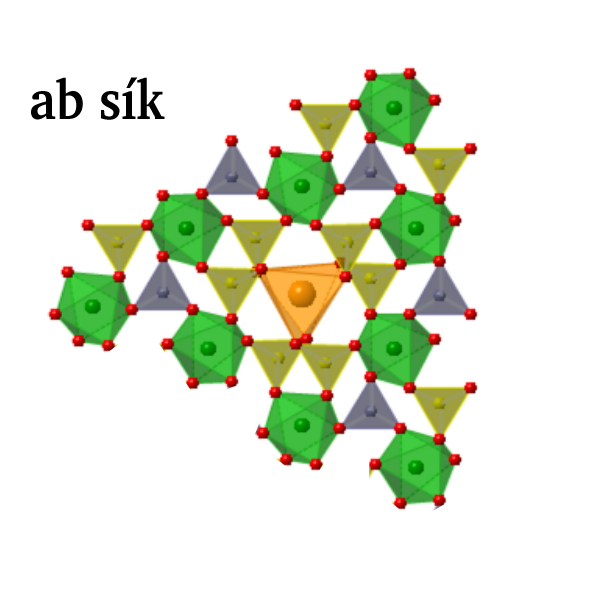
\includegraphics[width=\linewidth]{kristaly/homogenspin (1) (2).png}


\end{subfigure}
\begin{subfigure}[b]{0.4\linewidth}
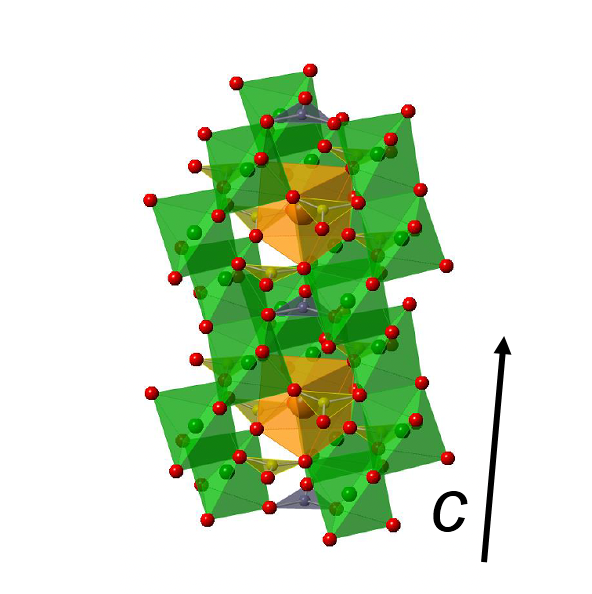
\includegraphics[width=\linewidth]{kristaly/struct (1).png}


\end{subfigure}

$\quad\textcolor{narancs2}{\blacksquare}\,$ Sm, $\quad\textcolor{zold2}{\blacksquare}\,$ Fe, $\quad\textcolor{citrom}{\blacksquare}\,$ $\textcolor{szurke}{\blacksquare}\,$ B

\caption{$\mathrm{SmFe_3(BO_3)_4}$ kristályszerkezete \cite{2018_PRL}, }
\label{fig:kristalyszerk}
\end{figure}

\subsection{A \texorpdfstring{$\bm{\mathrm{SmFe_3(BO_3)_4}}$}{TEXT} mágneses tulajdonságai \label{magnch}}

A ritkaföldfém-vas-borátokban Fe$^{3+}$ ionok $S$=5/2 spinjei antiferromágnesesen rendeződnek $30-40\,$K alatt. Az egytengelyű mágneses anizotropia előjelét a ritkaföldfém ionok fajtája határozza meg: a könnyű-tengelyű (easy-axis) vegyületekben, pl. $\mathrm{TbFe}_3(\mathrm{BO}_3)_4$, a momentumok a $c$ tengellyel párhuzamosan, míg a könnyű-síkú (easy-plane) változatokban, pl. $\mathrm{SmFe}_3(\mathrm{BO}_3)_4$, arra merőleges síkban helyezkednek el. Az általam vizsgált $\mathrm{SmFe}_3(\mathrm{BO}_3)_4$ esetén, a Hund-szabályok alapján, a $\mathrm{Sm}^{3+}$ ionok 5 db 4f elektronjának spin és pályamomentumai: $S$=5/2 és $L$=5, melyből a teljes pályamomentum $J$=5/2. Ezt az elektronállapotot a spektroszkópiában a $^6H_{5/2}$ szimbólummal jelöljük, amely a következőképpen adja meg az  impulzusmomentumokat $^{2S+1}L_J$.





 \begin{figure}[H]
\begin{center}
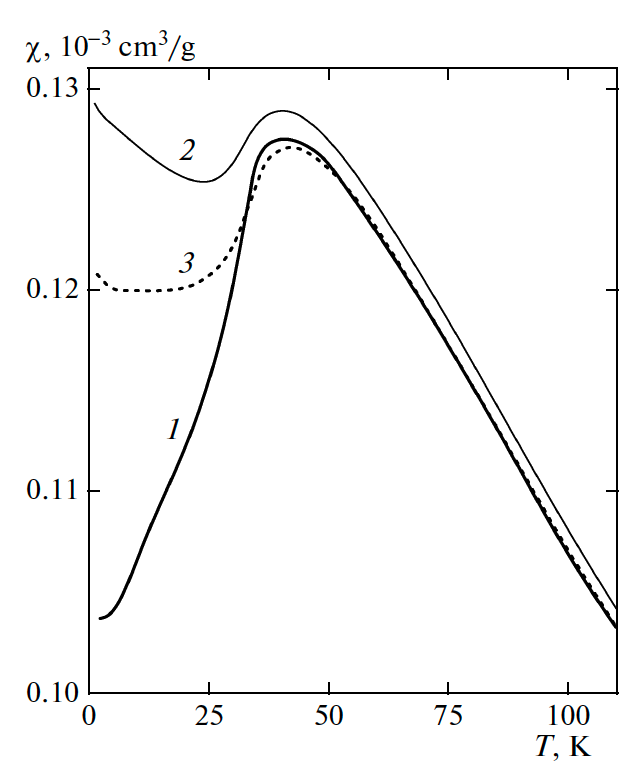
\includegraphics[width=7 cm]{kristalymágnesestul/szucc.png}
\end{center}
\caption {A $\mathrm{SmFe_3(BO_3)_4}$ mágneses szuszceptibilitásának hőmérsékletfüggése \cite{2010_JETP}. A kristály mágnesezettségét (M) mérték $H=$ 1\,kOe nagyságú, $c$ tengelyre merőleges (1) és párhuzamos (2) $H$ mágneses térerősség esetén, a szuszceptibilitás ennek mágneses tér szerinti deriváltja. A (3)-as görbe a $H\approx$ 10\,kOe nagyságú mágneses térerősség esetén történő mérés eredménye, ahol a mágneses tér hatására újrarendeződnek a vas ionok spinjei az $ab$ síkban, és merőlegesek lesznek a mágneses mezőre.}
\label{fig:szucc}
\end{figure}


A $\mathrm{SmFe_3(BO_3)_4}$ paramágneses fázisában a szuszceptibilitás közel izotróp (\ref{fig:szucc}. ábra) és követi a Curie-Weiss törvényt. Körülbelül 40\,K alatt a szuszceptibilitás csökkeni kezd, majd anizotroppá válik $T_N\approx33\,\mathrm{K}$ körül \cite{2010_JETP}. A $c$ tengelyre merőleges irányban mért szuszceptibilitás lényegesen gyorsabban csökken alacsony hőmérsékletek felé, mint a $c$ tengellyel párhuzamos komponens, mely könnyű-síkú anizotrópiára utal. A szuszceptibilitás anizotrópiáját a momentumok irányfüggő eloszlása határozza meg, amit a $c$ tengelyre merőleges síkbeli trigonális anizotrópia és/vagy az  indukált magneto-elasztikus anizotrópia szabnak meg. $H\approx$ 10\,kOe nagyságú mágneses térerősség hatására a spinek a síkon belül elfordulnak és merőlegesen állnak be a térerősségre, mely egy átlagos transzverzális szuszceptibilitást eredményez. 

A  ${\mathrm{SmFe_3(BO_3)_4}}$ mágneses szerkezetét neutronszórási kísérlettel határozták meg \cite{2012_JPhys}. A mágneses szerkezet meghatározásához a feltételezett szerkezet szabad paramétereit illesztik a mért diffrakciós mintázatra. Ehhez a finomításhoz felhasználták a ${\mathrm{SmFe_3(BO_3)_4}}$ ionok  mágneses formfaktorait. A vas ionok mágneses momentumai ferromágnesesen rendeződnek egy $ab$ síkbeli rétegen belül úgy, hogy $c$ irányban a rétegek között viszont antiferromágneses rendeződés van. A finomításnál használt első modellben a Sm és a Fe spinjei párhuzamosak egymással. Az illesztésből meghatározott mágneses momentumok nagysága,   $1.7 $ K-en, $\mu_{\mathrm{Fe}}=4.2(1) \mu_{\mathrm{B}}$ és $\mu_{\mathrm{Sm}}=0.24(4) \mu_{\mathrm{B}}$ \cite{2012_JPhys}. 

A modell további finomítása szerint a Fe és a Sm mágneses momentumai kb. 70$^\circ$-kal vannak elforgatva egymáshoz képest (lásd \ref{fig:magnszerk}. ábra) $\mu_{\mathrm{Fe}}=4.2(1) \mu_{\mathrm{B}}$ és $\mu_{\mathrm{Sm}}=0.8(2) \mu_{\mathrm{B}}$. A finomítást tovább analizálva azt találták, hogy minden modell, amiben a Sm teljes momentuma($\mu_{\mathrm{Total }}$) $0.5 \mu_{\mathrm{B}}<\mu_{\text {Total }}<1.4 \mu_{\mathrm{B}}$ tartományba esik, hasonlóan jól leírja a diffrakciós mérések eredményeit, így a Sm momentuma bizonytalan. Minden esetben a $90^\circ$ és $60^\circ$ közötti dőlés jobban preferált, mint a kollineáris párhuzamos elrendezés. A ${\mathrm{SmFe_3(BO_3)_4}}$ neutronszórás kísérletekből meghatározott mágneses struktúrája a \ref{fig:magnszerk} ábrán látható. A szamárium helyek mágneses momentumait, a jobb láthatóság érdekében, kétszer akkorának ábrázolták.




   \begin{figure}[H]
\begin{center}
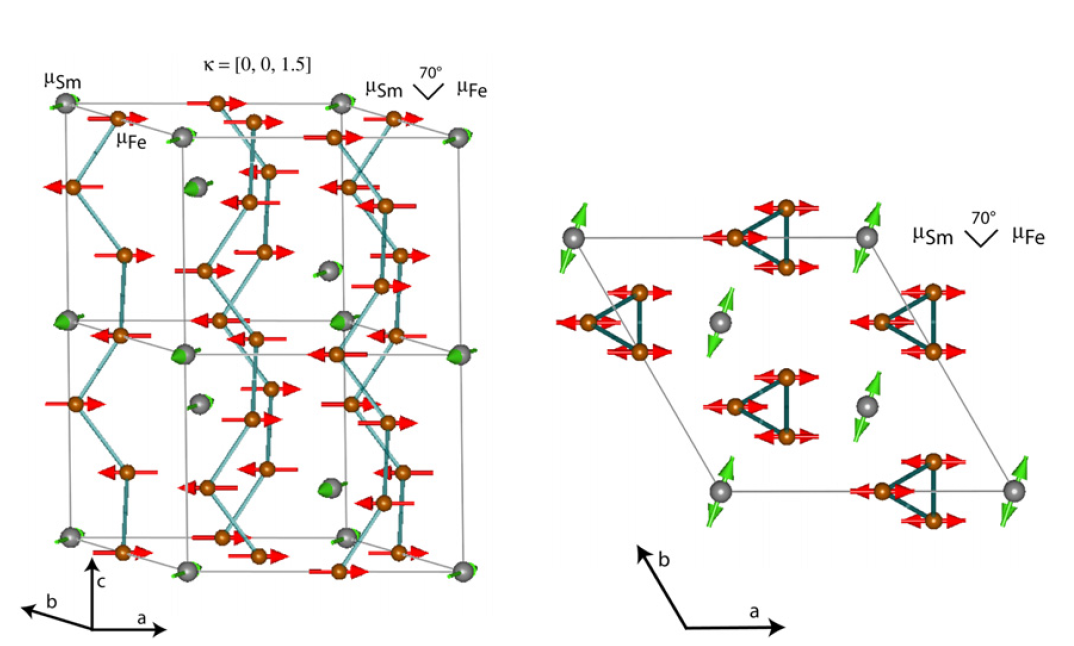
\includegraphics[width=\linewidth]{mágneses szerkezet/magnszerk.png}
\end{center}
\caption{
  ${\mathrm{SmFe_3(BO_3)_4}}$ mágneses szerkezete. A Sm-momentumok zöld színnel és a Fe-spinek pirossal vannak jelölve. A direkt Fe-Fe kicserélődéseket a helikális láncok mentén világos kék vonalak jelölik. Balra: elemi cellák megduplázódása a c-irányban. Jobbra: a Sm és a Fe alrácsok közötti elfordulás a $c$ tengely felőli síkból szemlélve. 
\cite{2012_JPhys} }

\label{fig:magnszerk}
\end{figure}


A ritkaföldfém-vas-borátok királis kristályszerkezetük miatt magnetoelektromos effektust mutatnak, ahol a külső mágneses tér elektromos polarizációt indukál bennük. Az időtükrözési és az inverziós szimmetria megsértése szükséges a magnetoelektromos csatolás megjelenéséhez. Vas-borátok esetén a könnyű-síkú anizotrópia nagyobb polarizációt eredményez, mint a könnyű-tengelyű anizotrópia. Az antiferromágneses domének átrendeződése kis mágneses térben gyors növekedést eredményez a polarizáció és magnetostrikció számára. A mágneses tér orientációjától függően előjelet válthat a polarizáció. A magnetoelektromos polarizáció előjelet váltásának kritikus értékét a ritkaföldfém ion Zeeman-energiája és a Fe-R kicserélődési kölcsönhatás aránya határozza meg.



 \subsection{\texorpdfstring{$\bm{\mathrm{SmFe_3(BO_3)_4}}$}{TEXT} THz abszorpciójának mágneses és elektromos terekkel történő vezérlése \label{ch:2.3}}


 
 
 ${\mathrm{SmFe_3(BO_3)_4}}$ csatolt Fe-Sm antiferromágneses rezonanciáját $10\,\mathrm{cm}^{-1}$ terahertz (THz) transzmissziós spektroszkópiával detektálták \cite{2018_PRL}. A különböző fénypolarizáció mellett végzett abszorpciós mérésekből meghatározták, hogy a rezonancia mágneses dipól-aktív, és az antiferromágneses \textbf{L} vektorra merőleges oszcilláló mágneses mezővel gerjeszthető.
 

\begin{figure}[H]
\begin{center}

\begin{subfigure}[b]{0.2\linewidth}
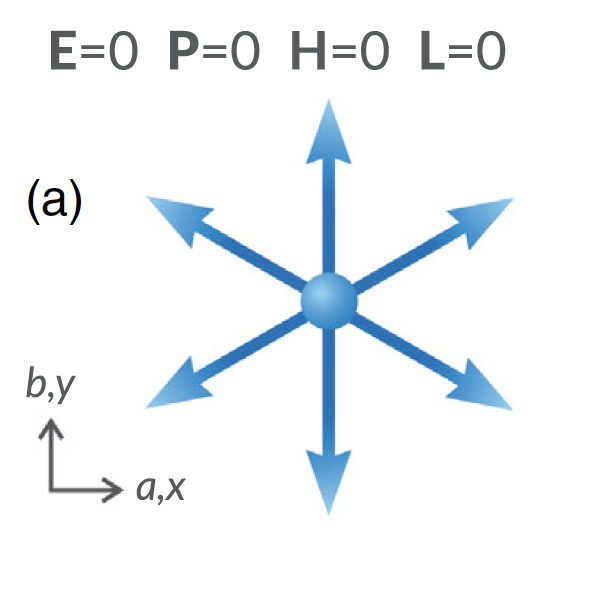
\includegraphics[width=\linewidth]{Dávidék mérései/homogenspin.png}
\end{subfigure}~%
\begin{subfigure}[b]{0.6\linewidth}
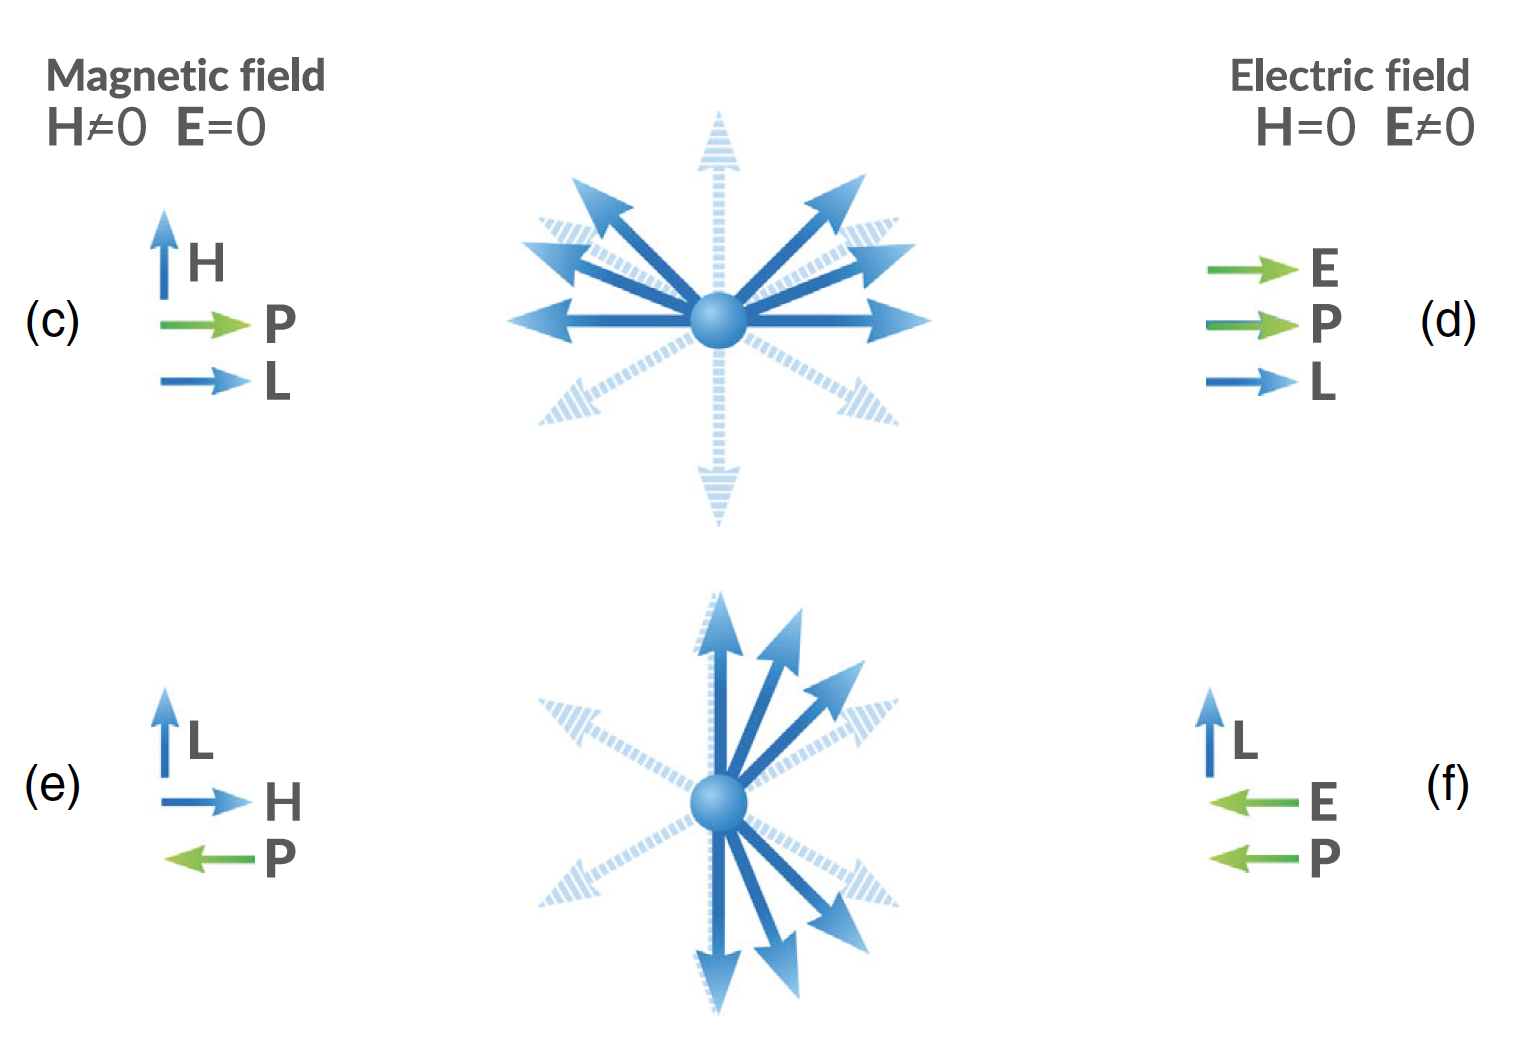
\includegraphics[width=\linewidth]{Dávidék mérései/spinE-B.png}

\end{subfigure}

\end{center}
\caption{Elektromos és mágneses rendeződés ritkaföldfém-vas-borátokban.\\ (a) Fe spinek (kék nyilak) homogén eloszlása az $a b$ síkban, állandó mágneses $(\mathbf{H})$ és elektromos $(\mathbf{E})$ tér hiányában. A nyilak a minta különböző doménjeit reprezentálják. Ebben az esetben mind az $\mathbf{L}$ antiferromágneses vektor mind pedig $\mathbf{P}$ az eredő statikus polarizáció nulla. $\mathbf{H} \parallel b$ mágneses mező (c) és  $\mathbf{E} \uparrow \uparrow a$ elektromos tér (d) által indukált $\mathbf{P} \uparrow \uparrow a$ és $\mathbf{L} \parallel a$. A mágneses tér 90$^\circ$-al történő elfordítása $\mathbf{H} \parallel a$ irányba (e), vagy az elektromos tér előjelének megfordítása $\mathbf{E} \uparrow \downarrow a$ (f) a statikus polarizáció és antiferromágneses vektor irányának felcserélését eredményezi \cite{2018_PRL}.}
\label{fig:spinszerk}
\end{figure}

\ref{fig:spinszerk}a. ábrán látható, hogy külső mágneses tér nélkül a lokális mágneses momentumok homogén módon oszlanak el az $ab$ síkban. Ez azt jelenti, hogy átlagosan a mágneses momentumok 50\%-át gerjeszti az $ab$ síkban lineárisan polarizált elektromágneses sugárzás. Ez nagy mértékben megváltozik, ha mágneses vagy elektromos térbe helyezzük a mintát. Ahogy a \ref{fig:spinszerk}c--f. ábrákon látható a külső terek megszüntetik a mágneses momentumok homogén eloszlását az $ab$ síkban. Ez egyrészt az antiferromágneses rend mágneses szuszceptibilitás anizotrópiájának illetve az előző fejezet \eqref{eq:1}-es képletével tárgyalt magnetoelektromos csatolásnak köszönhető. A külső mágneses illetve elektromos terek megtörik az $ab$ sík izotrópiáját és inhomogénné teszik a domének eloszlását. Ennek következtében  a módus intenzitását megváltoztatják, anizotróppá teszik. A \ref{fig:magnonB}a. és a \ref{fig:magnonB}b. ábrák azt demonstrálják, hogy a módus erőssége vagy csökkenthető, vagy növelhető, a külső mágneses tér irányától függően.


\begin{figure}[H]
\begin{center}
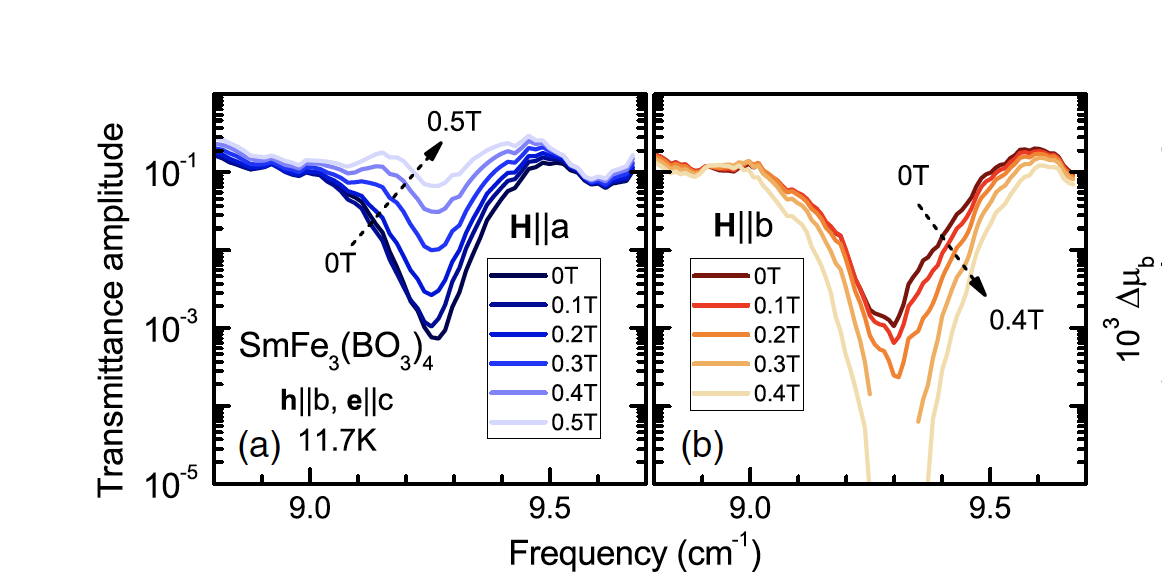
\includegraphics[width=10 cm]{Dávidék mérései/magnonmanipulationB.png}
\end{center}
\caption{Magnon gerjesztés manipulációja mágneses térrel. 
(a) A magnon gerjesztés intenzitásának csökkentése $a$ tengely irányú külső mágneses térrel. (b) Módus intenzitásának növekedése $b$ tengellyel párhuzamos mágneses térrel.
\cite{2018_PRL} }

\label{fig:magnonB}
\end{figure}

Ezen felül az alacsony kristályszimmetria következtében a ${\mathrm{SmFe_3(BO_3)_4}}$ lineáris dikroizmust mutat. Dikroizmusnak azt a jelenséget nevezzük, amikor két azonos frekvenciájú, de valamilyen tulajdonságban (esetünkben a fény polarizációban) eltérő foton állapotok abszorpciója eltér. A lineáris dikroizmus esetén két egymásra ortogonálisan polarizált állapot abszorpciója eltér.

\newpage

\section{Kutatásom közvetlen előzményei}

${\mathrm{SmFe_3(BO_3)_4}}$-on már BSc alatt is végeztem méréseket. A szakdolgozatomban a minta lineáris dikroizmusát vizsgáltam optikai spektroszkópiával látható és közeli infravörös tartományokban, illetve ennek hőmérsékletfüggését. Ezen kívül megkíséreltem a minta antiferromágneses doménjeinek befolyásolását külső elektromos és mágneses terekkel. Ezek a mérések a (\ref{fig:szakdoga}.) ábrán láthatóak.


\begin{figure}[H]
  \centering

  \begin{subfigure}[b]{0.28\textwidth}
  
    \caption*{$\bm{a)}$}
    \centering
    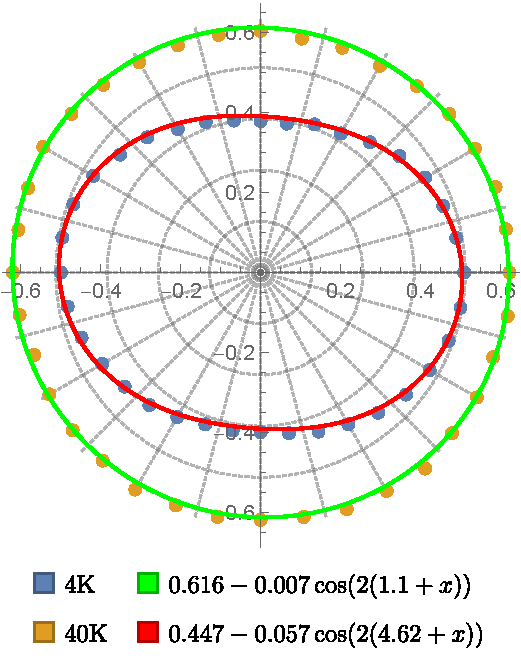
\includegraphics[width=\textwidth]{polforg_fit3.pdf}
  \end{subfigure}
  \hfill
  \begin{subfigure}[b]{0.48\textwidth}
  \caption*{$\bm{b)}$}
    \centering
    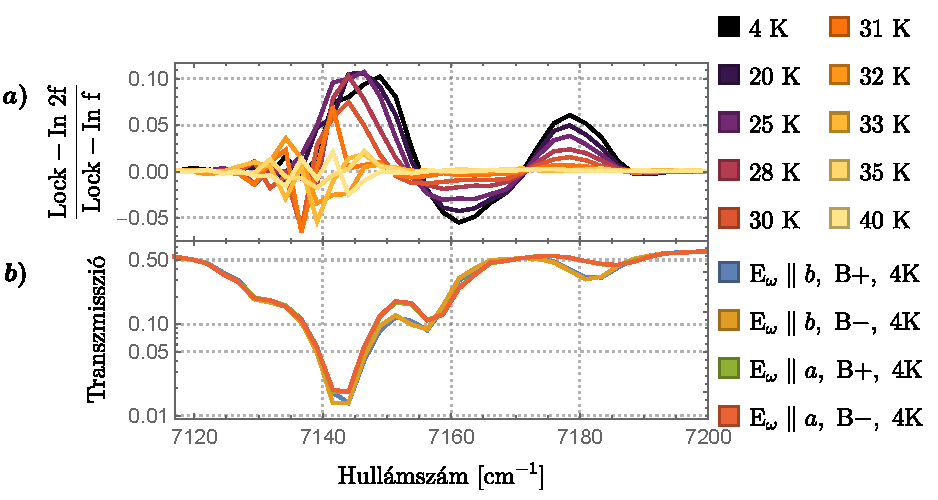
\includegraphics[width=\textwidth]{sajatmeresek/18-as2esabrkisint.pdf}
  \end{subfigure}
  
  \vspace{-4pt} % Adjust the vertical spacing between the subfigures and the third figure
  
   \begin{subfigure}[b]{0.48\textwidth}
    \caption*{$\bm{c)}$}
    \centering
    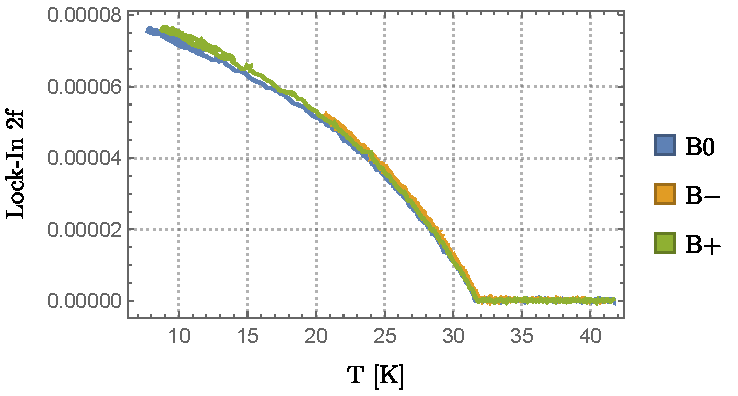
\includegraphics[width=\textwidth]{sajatmeresek/tsweep_2.pdf}
  \end{subfigure}
  \hfill
  \begin{subfigure}[b]{0.48\textwidth}
  \caption*{$\bm{d)}$}
    \centering
    \includegraphics[width=\textwidth]{sajatmeresek/Képernyőfotó 2023-06-02 - 19.01.10.png}
  \end{subfigure}
  
  \caption{Szakdolgozat keretein belül készített mérések. a) A minta transzmissziója a beeső lineárisan polarizált fénynyaláb polarizációs síkja szögének függvényében, b) A lineáris dikroismus hőmérsékletfüggése, c) Nagy frekvenciás lock-in mérés különböző mágneses terek esetén, d)Transzmissziós spektrumok az $^6F_{5/2}$ és $^6F_{11/2}$  f-f átmenetek közelében 4 K-en, mágneses és elektromos terek mellett}
  \label{fig:szakdoga}
\end{figure}

Az a) ábra jól szemlélteti a dikroizmust, b) esetben megfigyelhető hogy a dikroizmus jel amplitúdója csökken növekvő hőmérséklettel, és csak az antiferromágneses fázisban van jelen. c) a lineáris dikroizmus lockin technikával 930 nm hulámhosszon mért részletes hőmérsékletfüggése látható. Ezt követően a d) mérésben külső elektromos és mágneses terekkel próbáltam a minta antiferromágneses doménjeit rendezni, de az alkalmazott kis terekkel ez nem sikerült.



Ezt követően a TDK munkám keretein belül Terahertz spektroszkópiával vizsgáltam az anyag spingerjesztéseit külső mágneses térben és anélkül, illetve kiszámítottam az anyag törésmutató és abszorpciós együttható spektrumát. Ezek a következő ábrán láthatóak:

\begin{figure}[H]
  \centering

  \begin{subfigure}[b]{0.43\textwidth}
  
    \caption*{$\bm{a)}$}
    \centering
    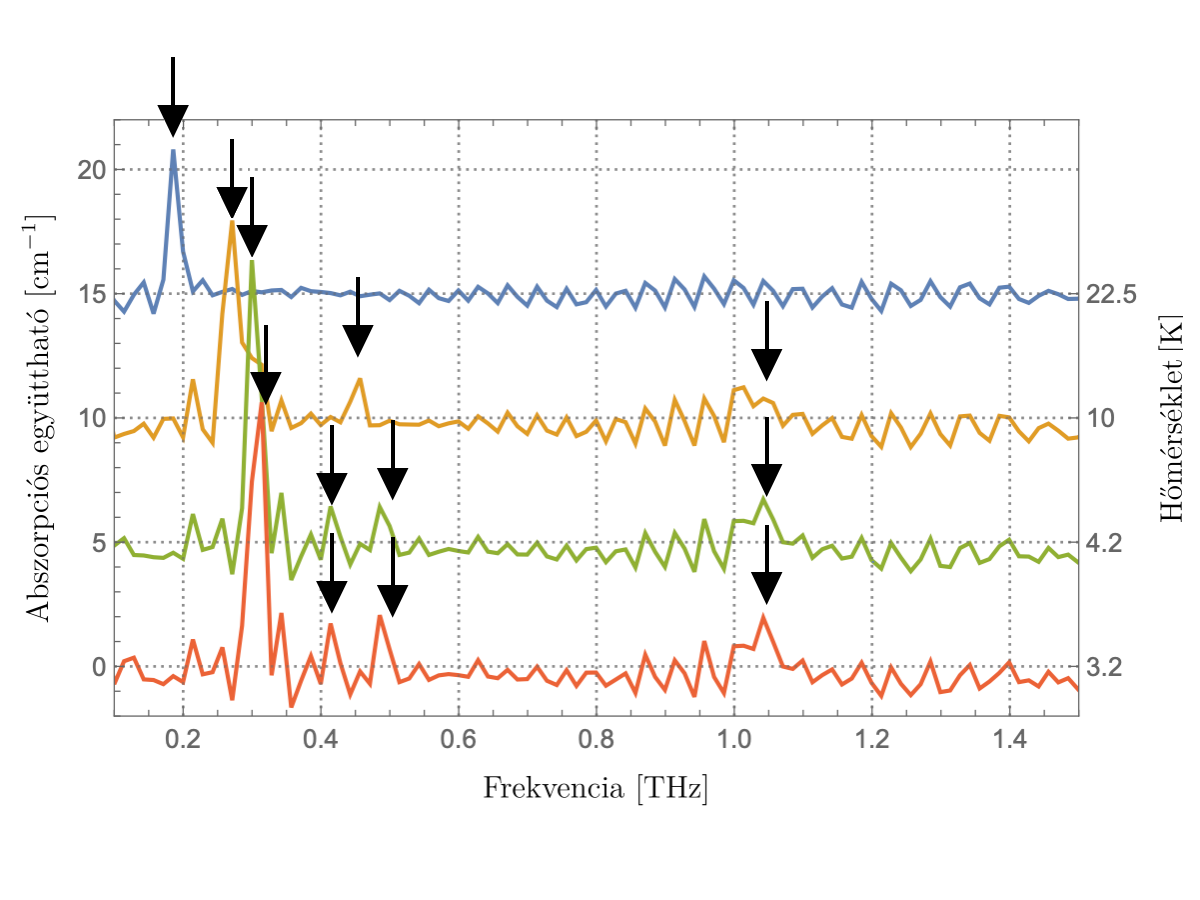
\includegraphics[width=\textwidth]{sajatmeresek/ov (2).png}
  \end{subfigure}
  \hfill
  \begin{subfigure}[b]{0.53\textwidth}
  \caption*{$\bm{b)}$}
    \centering
    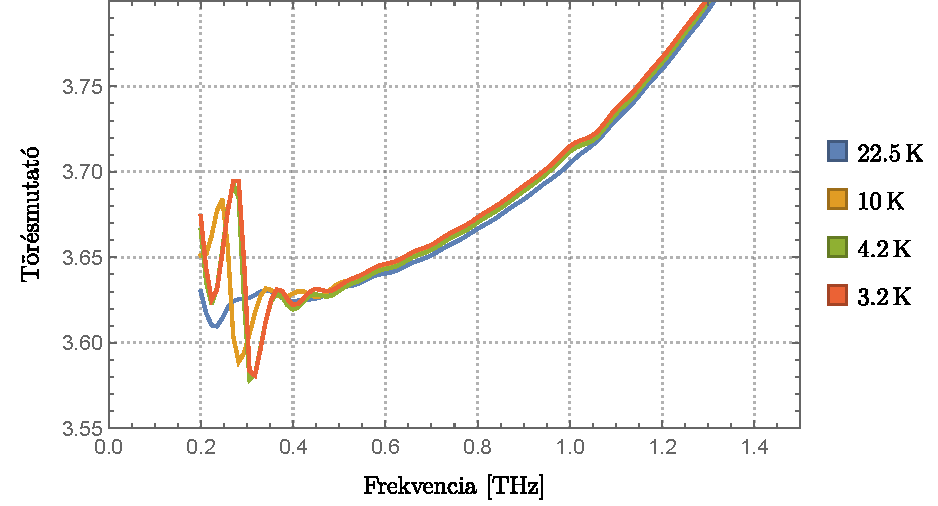
\includegraphics[width=\textwidth]{sajatmeresek/tores1 (1).pdf}
  \end{subfigure}
  
  \caption{TDK dolgozat keretein belül készített mérések. a) A minta spingerjesztéseinek hőmérsékletfüggése, b) A minta törésmutató spektrumának hőmérsékletfüggése}
  \label{fig:tdk}
\end{figure}

Az a) ábrán pedig megfigyelhető hogy először a vas majd a Sm ionok rendeződnek ahogy hűlik az anyag, ezért látható egyre több abszorpciós csúcs. A szakirodalomban már ismertetett gerjesztések mellett (\ref{ch:2.3}) 1 THz frekvenciánál egy új mágneses rezonanciát sikerült azonosítanom. Ez a módus nem értelmezhető az anyag két Fe és két Sm mágneses alrácsot tartalmazó modelljében, így a szakirodalomban szereplőnél komplexebb mágneses szerkezetre utal. A b) mérésen látható ahogy a rezonancia frekvencia a hőmérséklettel eltolódik, illetve hogy magas frekvenciákon a fononmódusok dominálnak a törésmutató spektrumban. Kis mágneses térrel próbáltam a rezonancia amplitúdókat befolyásolni de ez nem bizonyult sikeresnek. Ebben a félévben pont ezért a minta nagy mágneses térben történő vizsgálatát tűztem ki célul, hogy a spingerjesztéseket, doméneket befolyásolni tudjam a \ref{ch:2.3}. fejezetben ismertetett méréseknek megfelelően, ezzel folytatva előző kísérleteimet. Ehhez egy nagy mágneses terű optikai kriosztát fejlesztése és a hozzá kapcsolódó THz optikai elrendezés kialakítása szükséges.\\
Az Önálló labor első félévében a laborba nemrég érkezett, használtan kapott nagy mágneses terű kriosztát fejlesztését és a hőszigetlő vákuumköpeny karakterizálását végeztem el. Először a meglévő mintatartó pálca végére terveztem új befogót, majd a kriosztát lefedett széles szögű ablakát alumínium lemezről spectrosilra cseréltem és ezzel végeztem próba méréseket.















 
 
 

%\section{DD, FF átmenetek}
\newpage
\section{Kísérleti módszerek, a mérések kiértékelése}



\subsection{Időfelbontásos terahertz spektroszkópia }
Az optikai spektroszkópia, az optikai tulajdonságok frekvenciafüggő vizsgálata fontos információt szolgáltat az anyagok összetételéről és szerkezeti felépítéséről. Míg az elektromágneses spektrum alacsony frekvenciás, mikrohullámú és infravörös tartománya régóta intenzíven kutatott terület, a kettő közötti, 100 GHz-től 10 THz-ig terjedő terahertz frekvenciatartomány csak a közelmúltban vált kísérletileg hozzáférhető, mivel korábban széles spektrumú források nem álltak rendelkezésre ebben a tartományban. Az egyciklusú, tehát a rezgésiidővel összemérhető pulzusszélességű THz pulzusok generálását és detektálását a femtoszekundumos (fs) lézerek elterjedése és a gyors fotokapcsolók kifejesztése alapozták meg. Ezen THz pulzusok pedig lehetővé tették az időfelbontásos THz spektroszkópia létrejöttét.\\

A kísérletek során alkalmazott mérési elrendezés a (\ref{fig:merelrend}) ábrán látható:

\begin{figure}[H]
\begin{center}


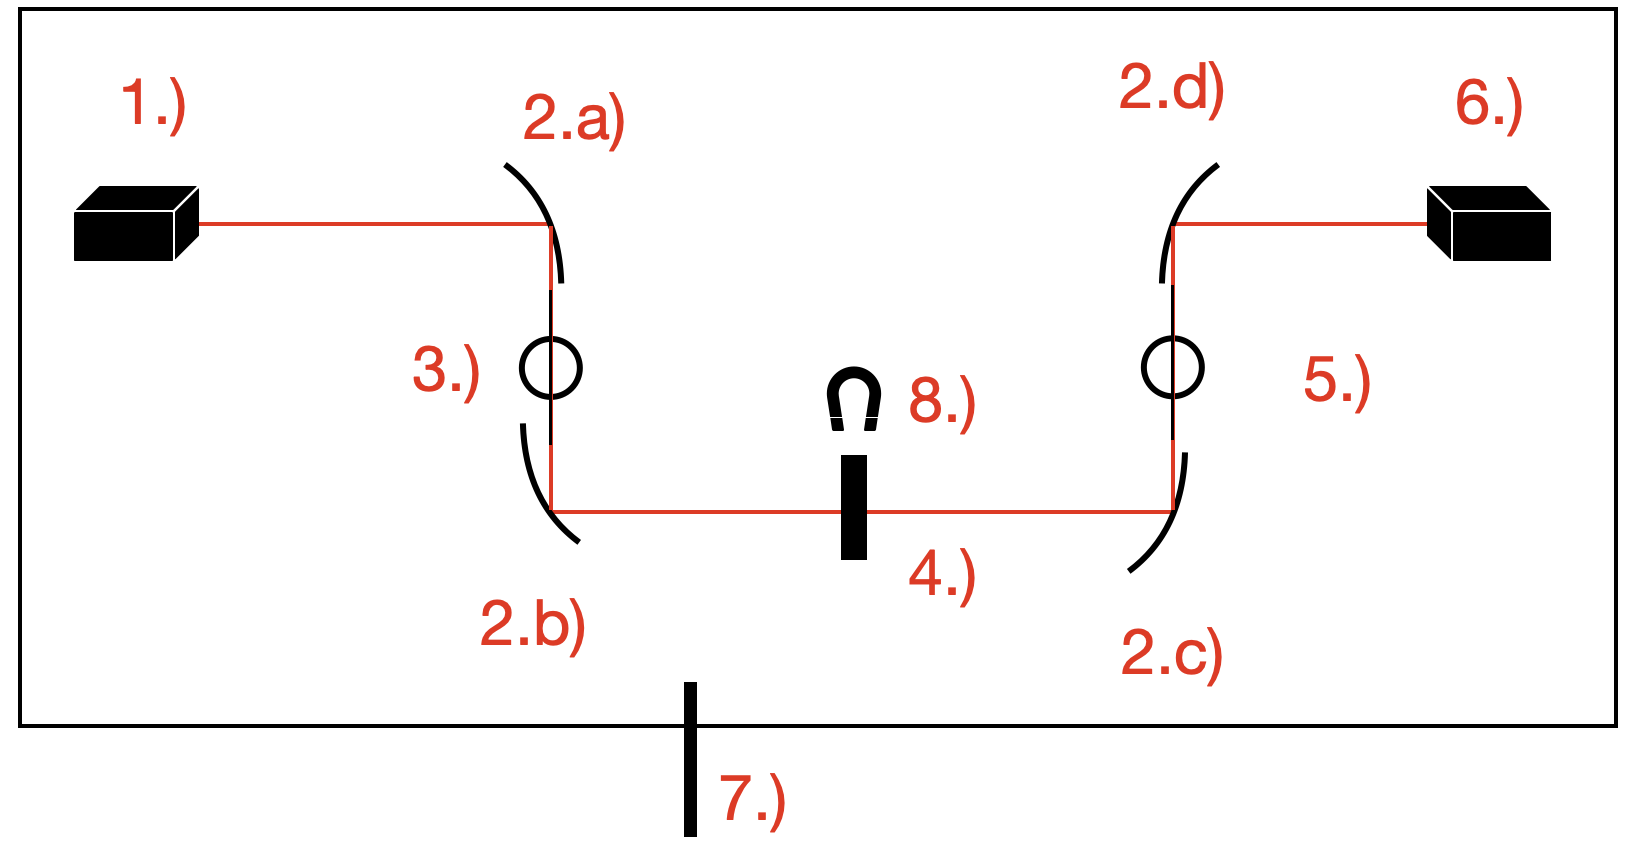
\includegraphics[width=\linewidth]{meresielrendezes/merelrendmagn.png}




\end{center}
\caption{A mérésekhez alkalmazott transzmissziós időfelbontott THz spektrométer. $\bm{a)}$ Az elrendezés sematikus rajza. 1.) és 6.) Ultrarövid időtartamú infravörös lézer impulzussal gerjesztett THz adó és vevő antennák. 2.) Parabola tükrök. 2.a,c) a pontforrásból széttartó nyalábot párhuzmosítja, 2.b,d) a párhuzamos nyalábot fókuszálja. 3.), 5.) Vékony párhuzamos drótokból álló (wire grid) polarizátorok. 4.)Optikai mágnessel felszerelt kriosztát. 7.) Szárazlevegő beáramló nyílása. Mérési elrendezés mágneses tér mellett is használható (8.)).}

\label{fig:merelrend}
\end{figure}





\subsection{Mérések kiértékelése}
A félév alatt méréseket csak a spectrosil üvegen végeztem de más minta esetén is ugyanaz lenne a mérések menete. Először rögzítem az elektromos tér időbeli változását majd ebből megállapítom az amplitúdó és fázis spektrumokat Fourier transzformáció segítségével. Ezt követően pedig az alábbi képleteket használva különböző spektrumokat készítek el.


\subsection{Törésmutató, dielektromos állandó és abszorpciós együttható számítása}

A kiértékeléshez 3 komplex Fourier-transzformáltat határozok meg:


\begin{equation*}\label{eq:1}
\begin{gathered}
T_1=\left |\frac{E_1}{E_{ref}}\right |,\quad T_3=\left |\frac{E_3}{E_{ref}}\right |, \quad T_{telj}=\left |\frac{E_{telj}}{E_{ref}}\right |
\end{gathered}
\end{equation*}

Ahol $E_{telj}$ a teljes mért jel Fourier-transzformáltja, $E_{1}$ és $E_{3}$ pedig a mintán áthaladó direkt nyaláb és a mintában visszaverődéseket szenvedő nyaláb Fourier-transzformáltjai. $E_{ref}$ a minta nélkül, a minta keresztmetszetével megegyező méretű és alakú referencia apertúrán végzett mérés Fourier-transzformáltja. A megfelelő $T_i$-k pedig az előbb említett jelek transzmissziói. Ahhoz hogy kiszámoljam a komplex törésmutatót($n$) a következő egyenleteket alkalmaztam \cite{NEMEC2005}:

\begin{equation}\label{eq:2}
T_1(n, z)=\frac{4 z}{(z+1)^2} \exp (2 \pi \mathrm{i}(n-1) f d / c)
\end{equation}

\begin{equation}\label{eq:3}
T_3(n, z)=T_1(n, z)\left(\frac{z-1}{z+1}\right)^2 \exp (4 \pi i n f d / c)
\end{equation}


Itt $f$ a frekvencia, $c$ a vákuumbeli fénysebesség, $d$ a minta vastagsága, $z$ pedig az úgynevezett felületi impedancia: $z = \sqrt{\frac{\mu}{\epsilon}}$. Ha a transzmissziók elegendően széles frekvenciatartományon vett frekvenciaátlagával számolunk, akkor \ref{eq:3} a következőképpen módosul feltéve, hogy $\mu \approx 1$: 

\begin{equation}\label{eq:4}
\sqrt{\frac{T_3(n, z)}{T_1(n, z)}}=\frac{1-z}{z+1}
\end{equation}

Az exponenciális tagból eredő oszcilláció a frekvenciátlagból kiesik. Ebből már a $z$ meghatározható, és $n = 1/z$. Ebből pedig: $\varepsilon = n^2$


Az abszorpciós együtthatót pedig a következő képlettel lehet megkapni a $d$ mintavastagság felhasználásával:

\begin{equation}\label{eq:5}
\alpha=-2\frac{1}{d}(\ln T_{telj})
\end{equation}

\subsubsection{Törésmutató meghatározása a többszörösen visszavert nyaláb  időkésleltetésének felhasználásával \label{sec:mas}}
Az előző pontban ismertetett módszer a $z$ felületi impedancia és az $n$ törésmutató meghatározására a mintán áthaladó direkt nyaláb és a minta-vákuum határfelületről kétszer visszavert nyaláb amplitúdójának arányán alapul. Ha a minta az adott frekvenciatartományban átlátszó, akkor ez csak a reflexiós együtthatótól függ, azaz a minta felületéről szolgáltat információt. A továbbiakban a THz spektroszkópia időfelbontását kihasználva egy alapvetően különböző módszert mutatok be, ami kizárólag a minta tömbi tulajdonságaiból kiindulva adja meg a minta anyagának törésmutatóját.\\

Meghatározzuk a mintán áthaladó direkt nyaláb és a minta-vákuum határfelületről kétszer visszavert  nyaláb jeleihez tartozó első csúcsok időpontját. Ennek a két időpontnak a különbsége $\delta t$. Tudjuk, hogy a fény ez idő alatt $\delta t \cdot c$ optikai úthosszat tesz , másrészt a két nyaláb úthosszkülönbsége a mintavastagság kétszerese, amiből kiszámolható a törésmutató.

\begin{equation}\label{eq:6}
    n = \frac{\delta t \cdot c}{2 d}
\end{equation}

\subsection{Törésmutató spektrum számítása fáziskülönbségekből}

A frekvencia függő törésmutató kiszámolható az abszorpció spektrumok hányadosából \ref{eq:7} alapján:

\begin{equation}\label{eq:7}
T_{1}\approx\alpha=\frac{A_D}{A_{ref}}=\frac{e^{i \frac{\omega}{c} N_{minta} d}}{e^{i \frac{\omega}{c} N_{ref} d}}=e^{i \frac{\omega}{c}(\underbrace{N_{minta}-N_{ref}}_{\Delta N=\Delta n+i \Delta k}) d}
\end{equation}

Itt $d$ a minta vastagsága, $c$ a fénysebesség. Mivel a referenciamérés egy a mintával azonos keresztmetszetű üres, vákuumban lévő apertúrán keresztül történik, a referencia törésmutatója 1, és így a minta törésmutató spektruma meghatározható: 

\begin{equation}\label{eq:8}
    n_{minta}=(\varphi_{minta}-\varphi_{ref})c/(d\cdot2\pi f)+n_{ref}
    \end{equation}

\newpage


\section{Eredmények diszkussziója}
\subsection{Mintatartó pálca tervezése}
Ahhoz hogy a mostani mintámat használni lehessen a mágnessel felszerelt optikai kriosztátban egy mintatartó pálcát kellett terveznem. A megvalósított verzió a (\ref{fig:palca}b) ábrán látható.



\begin{figure}[H]
  \centering

  \begin{subfigure}[b]{0.3\textwidth}
    \caption*{$\bm{a)}$}
    \centering
    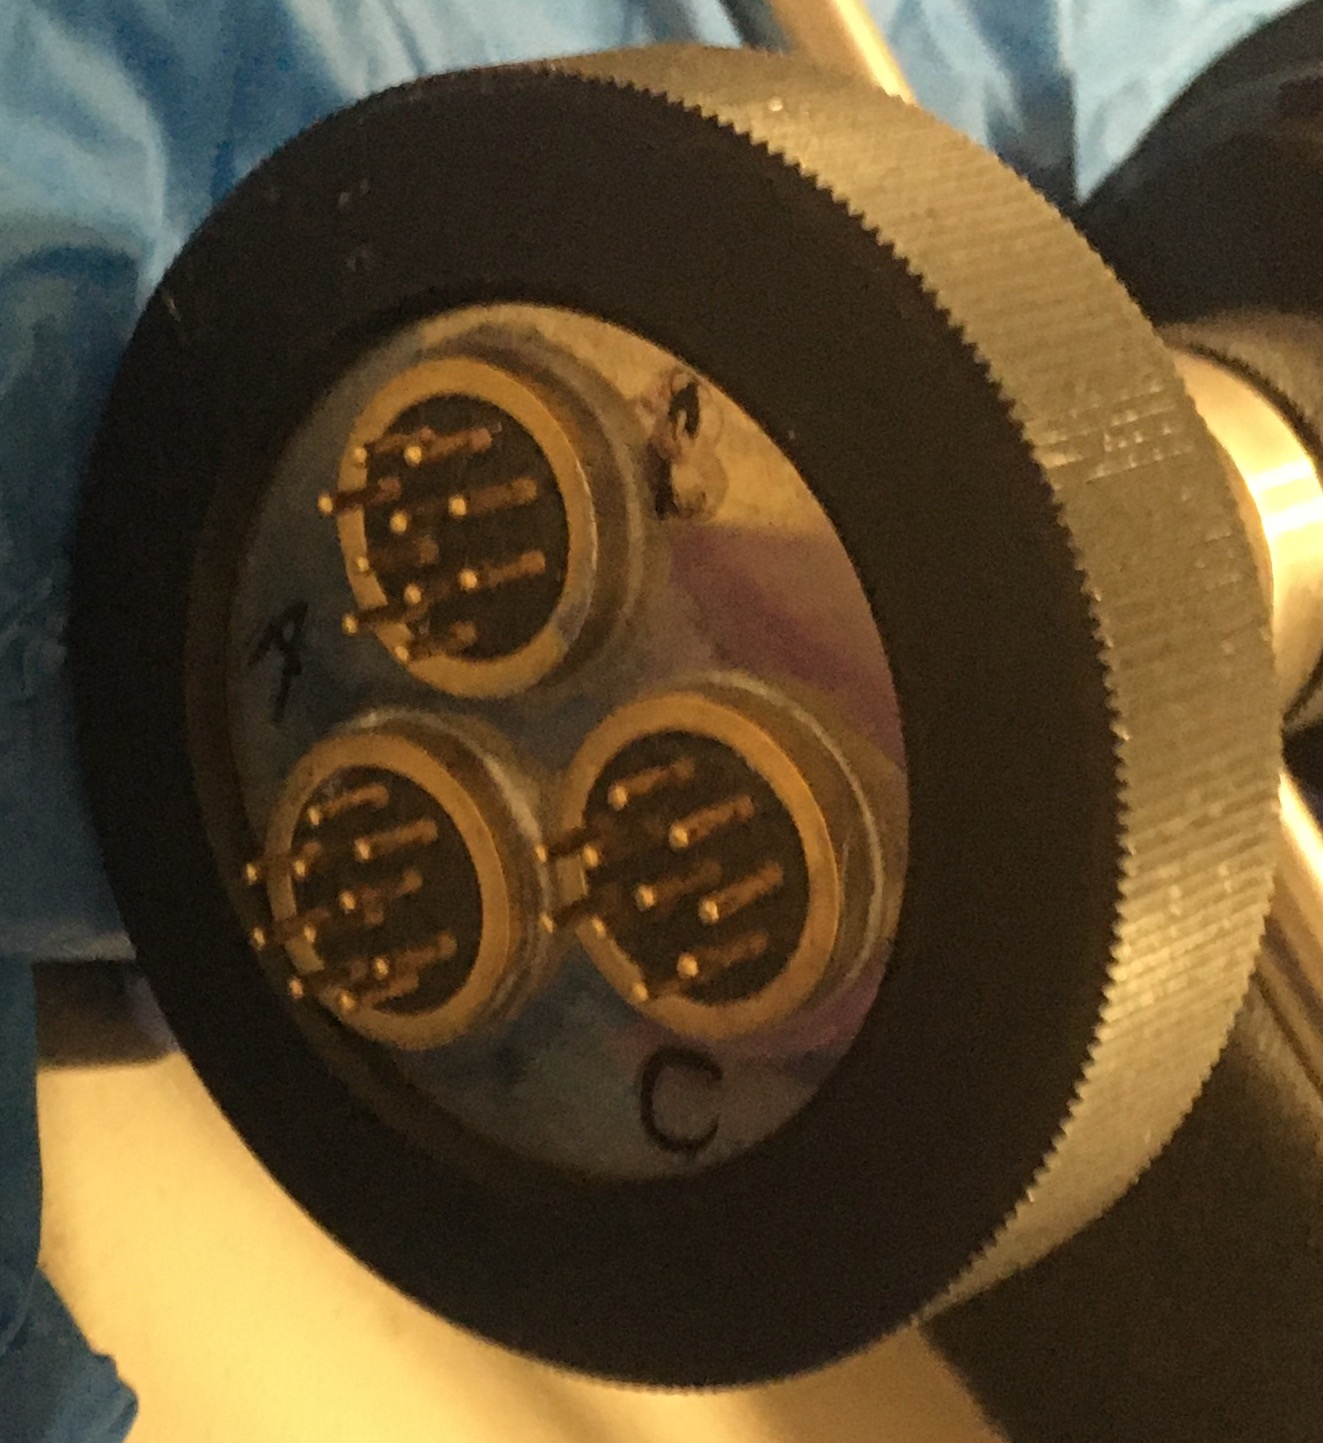
\includegraphics[width=\textwidth]{csat.JPG}
  \end{subfigure}
  \hfill
  \begin{subfigure}[b]{0.66\textwidth}
  \caption*{$\bm{b)}$}
    \centering
    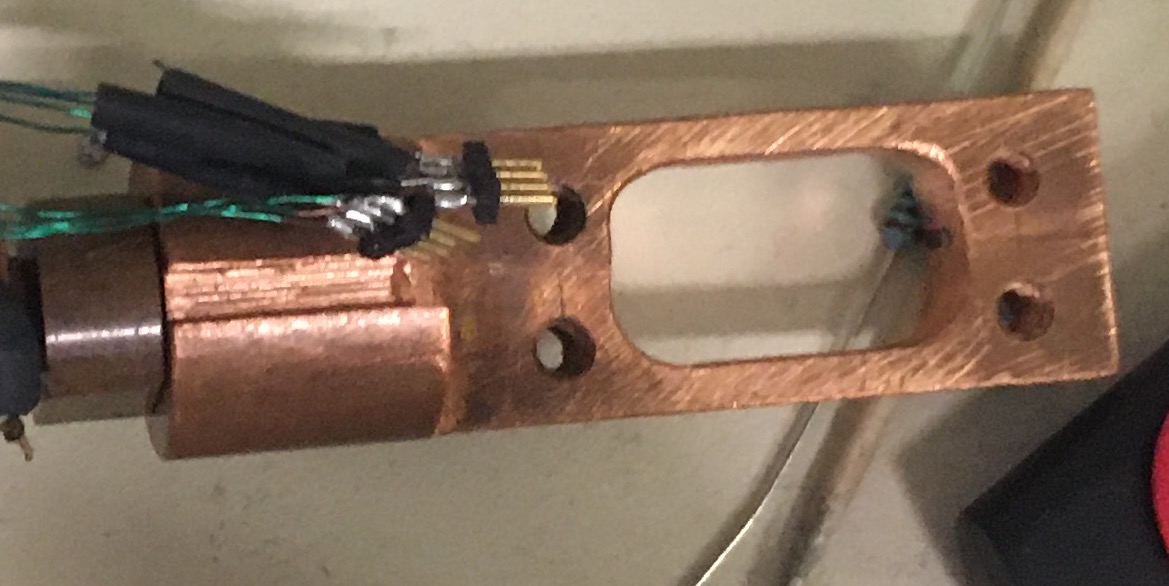
\includegraphics[width=\textwidth]{befogo.JPG}
  \end{subfigure}
  
  \vspace{-4pt} % Adjust the vertical spacing between the subfigures and the third figure
  
  \begin{subfigure}[b]{\textwidth}
  \caption*{$\bm{c)}$}
    \centering
    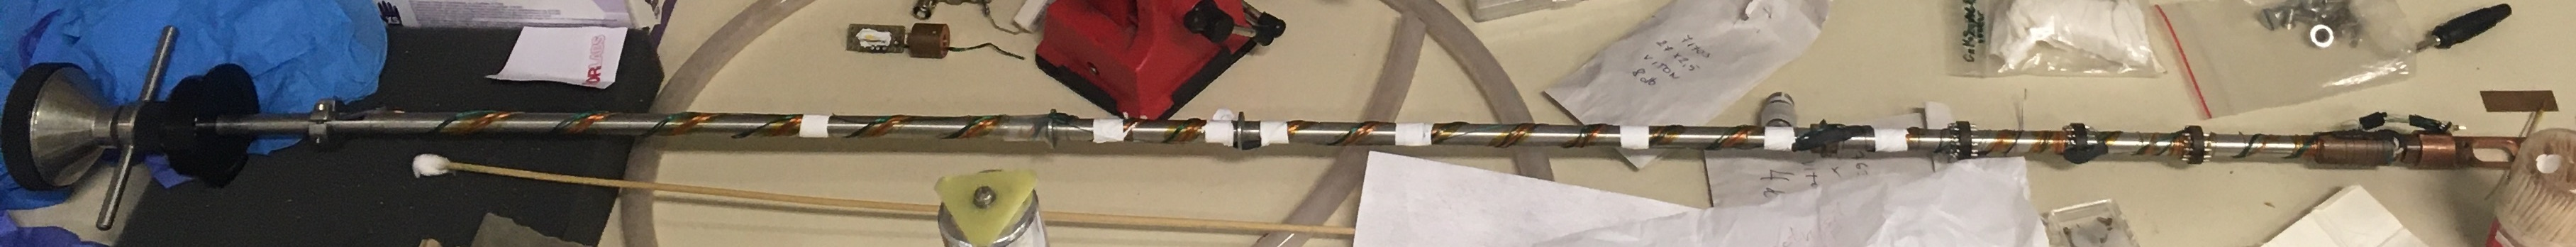
\includegraphics[width=\textwidth]{palcatelj.JPG}
  \end{subfigure}
  
  \caption{Mintatartó pálca, a) csatlakozók, b) mintabefogó tűsorokkal, c) teljes mintatartó pálca}
  \label{fig:palca}
\end{figure}

Nagyobb furatú mintabefogót terveztem a minta befogásához a nagyobb apertúrának köszönhetően a THz frekvenciatartományban is lehetséges jó jel-zaj viszonyú transzmisszióméréseket végezni. A befogó nyakán egy vájat lett kialakítva ahol a mintához közel elhelyezett Cernox-1050-es hőmérő vezetékeit lehet elhelyezni. A mintatartó nyakára nagy ellenállású (63 Ohm/m) ellenálláshuzalt tekercselek, amit fűtőellenállásként használva a minta hőmérséklete szabályozható. Az ellenálláshuzal és a hőmérő is a tűsoron keresztül csatlakozik a mérőpálca csatlakozóihoz. A mintatartó pálca a kriosztátban alacsony nyomású hélium gázban helyezkedik el, ami a kriosztát folyékony hélium fürdője és a minta közötti hőátadást biztosítja.

\subsection{Mintatartó lezáró alumínium lemezének spectrosil ablakra cseréje}

Ahogy az elméleti bevezetőben (\ref{ch:2.3}) is említettem, külső mágneses terekkel befolyásolható a minta spinrezonanciáinak amplitúdója. A mágneses térre merőleges (Voigt-geometria) és a mágneses térrel párhuzamos (Faraday-geometria) fényterjedés esetén is tervezek méréseket, amihez a kriosztát mind a négy ablakára szükség lesz, így az eddig alumínium lemezzel lezárt ablakát spectrosil üvegre cseréltem. Ezt megelőzően vizsgáltam a spectrosil THz frekvenciatartománybeli transzmisszióját (\ref{fig:transz1}). A jó tömítés érdekében alkalmaztam vákuumzsírt is a cserénél. A kriosztát és a kicserélt ablak a (\ref{fig:krio}.) ábrán látható. Az ablakcserét követően ellenőriztem a kriosztát hőszigetelő vákuumköpenyét. A műszerkönyvben szereplő 24 órás, turbómolekuláris pumpával történő vákuumozás után $1.2 \cdot 10^{-5}$\,mbar végvákuumot értem el, ami megfelelő a kriosztát kriogén folyadékokkal történő lehűtéséhez.

\begin{figure}[H]
  \centering

  \begin{subfigure}[b]{0.25\textwidth}
    \caption*{$\bm{a)}$}
    \centering
    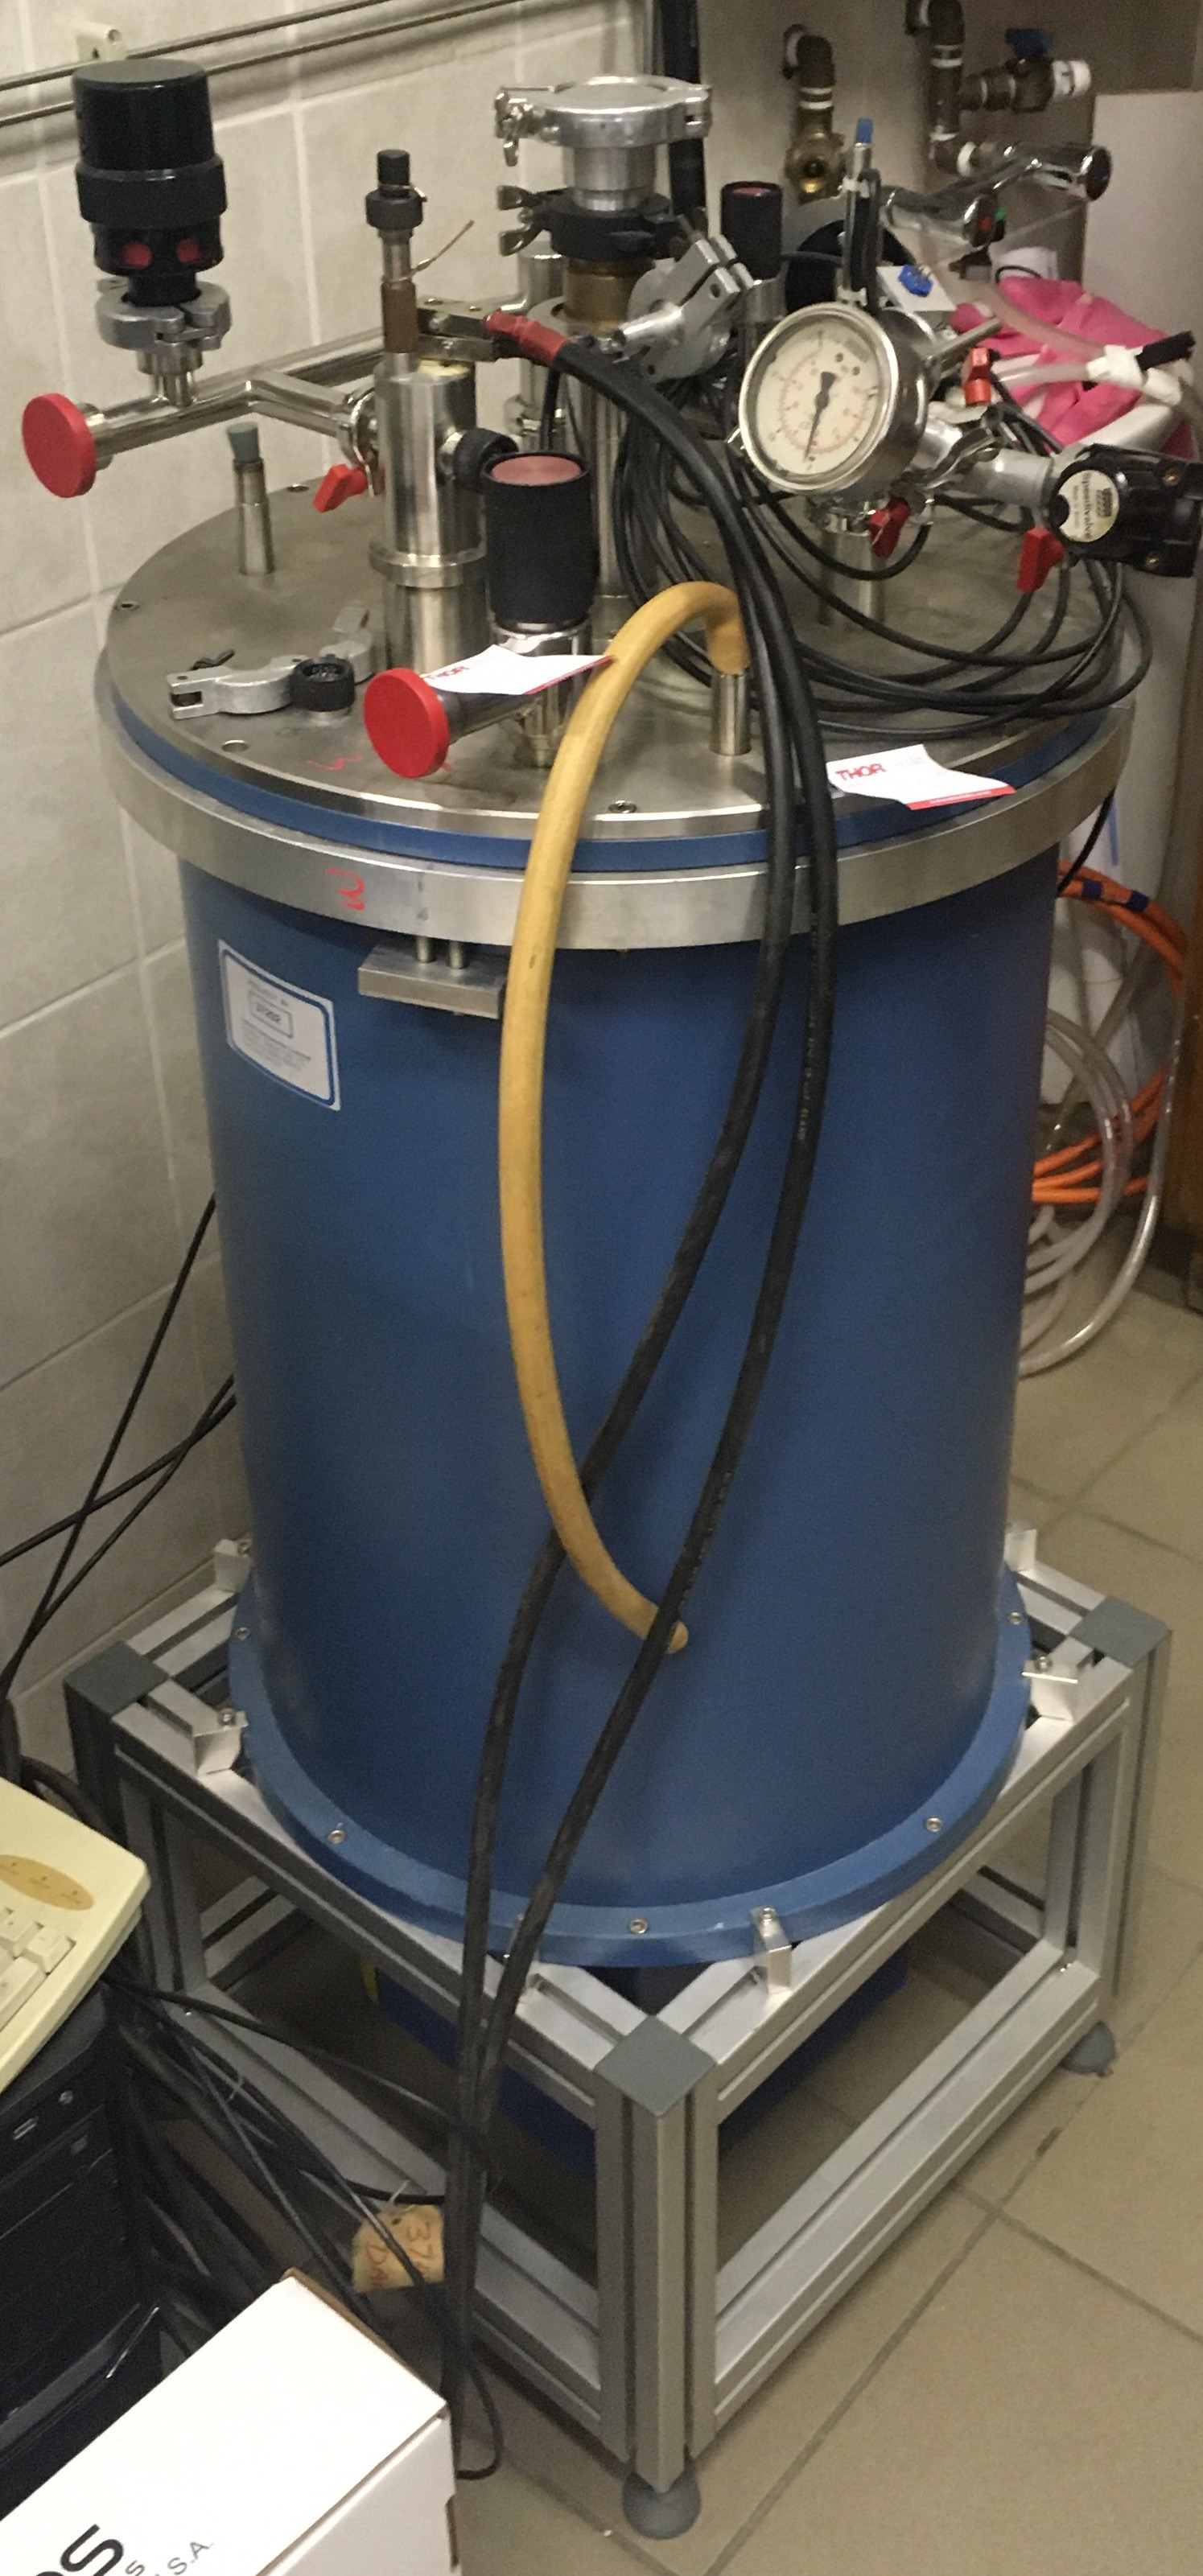
\includegraphics[width=\textwidth]{krio.JPG}
  \end{subfigure}
  \hfill
  \begin{subfigure}[b]{0.71\textwidth}
  \caption*{$\bm{b)}$}
    \centering
    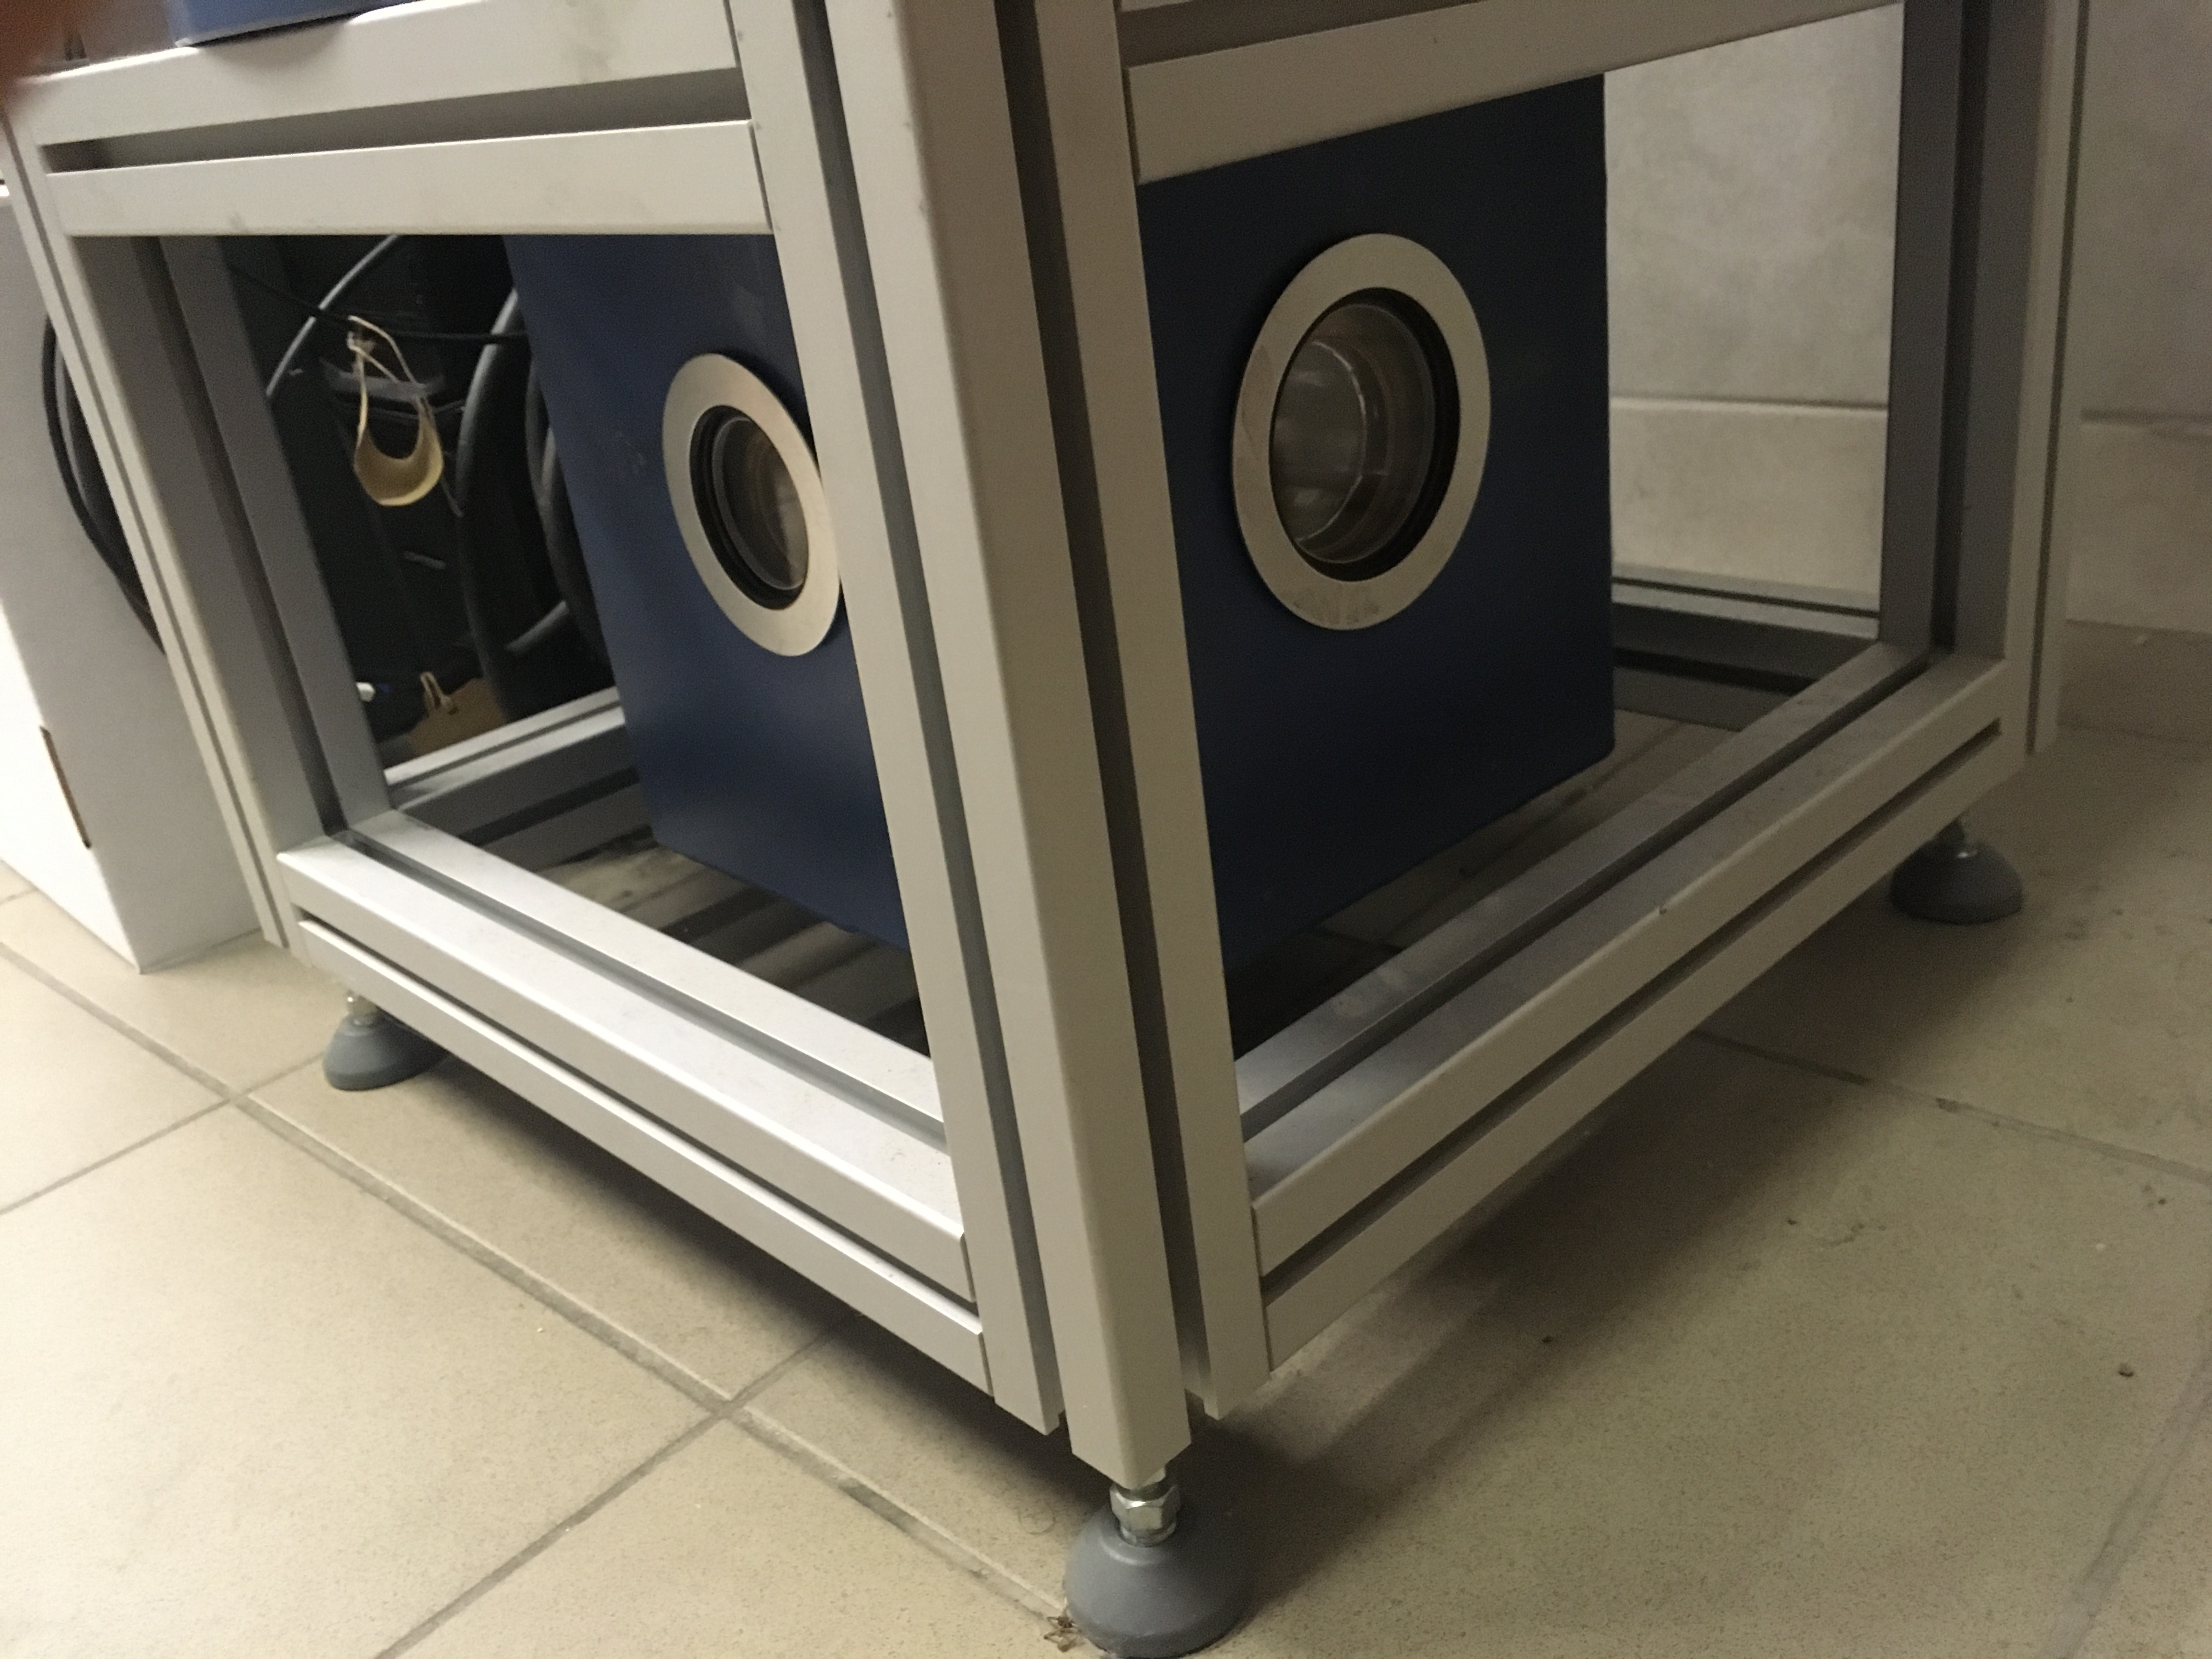
\includegraphics[width=\textwidth]{ablak1.JPG}
  \end{subfigure}
  
  \vspace{-4pt} % Adjust the vertical spacing between the subfigures and the third figure
  
  
  \caption{Oxford mágneses optikai kriosztát, a)A teljes kriosztát, a mérőpálcát a tetején lehet behelyezni a mintával együtt, b) belépő ablakok, a nagyobbik ablakot cseréltem alumíniumról spectrosilra}
  \label{fig:krio}
\end{figure}

Viszont még a beszerelés előtt a későbbi a mintán történő mérések kiértékeléséhez fontos a spectrosil ablak tulajdonságaival tisztában lenni ezért az ablakon végeztem méréseket szobahőmérsékleten. Megállapítottam az ablak transzmisszió abszorpció illetve törésmutató spektrumait. A mérések eredményei a következő ábrákon láthatóak.



\begin{figure}[H]
\begin{center}


\includegraphics[width=\linewidth]{beszamolo/időfüggő.pdf}




\end{center}
\caption{A transzmittált THz pulzus elektromos térerősségével arányos detektált jel időfüggése}

\label{fig:ido}
\end{figure}

\begin{figure}[H]
\begin{center}


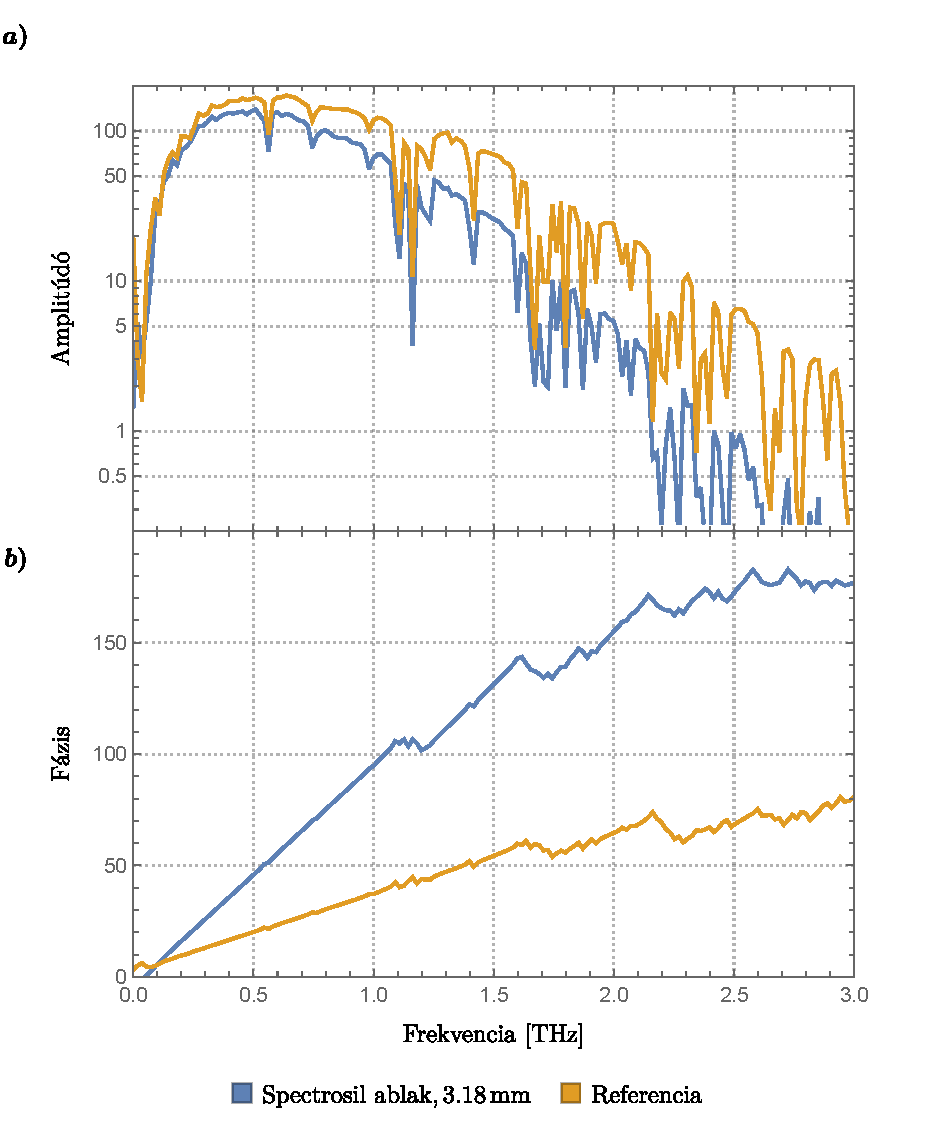
\includegraphics[width=\linewidth]{beszamolo/phaseampossz.pdf}




\end{center}
\caption{Fázis és amplitúdó spektrumok}

\label{fig:spektr}
\end{figure}






\begin{figure}[H]
\begin{center}


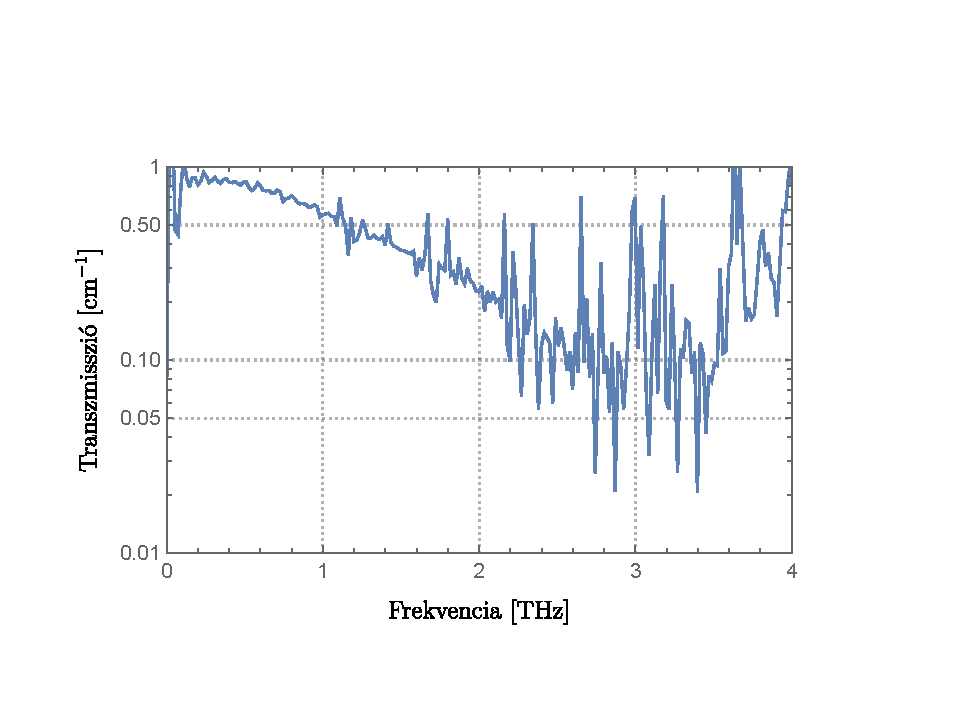
\includegraphics[width=0.9\linewidth]{beszamolo/transz1.pdf}




\end{center}
\caption{Számított transzmisszió spektrum}

\label{fig:transz1}
\end{figure}

A sok csúcs itt amit látni a levegőben lévő vízpára abszorpció vonalai.





\begin{figure}[H]
\begin{center}


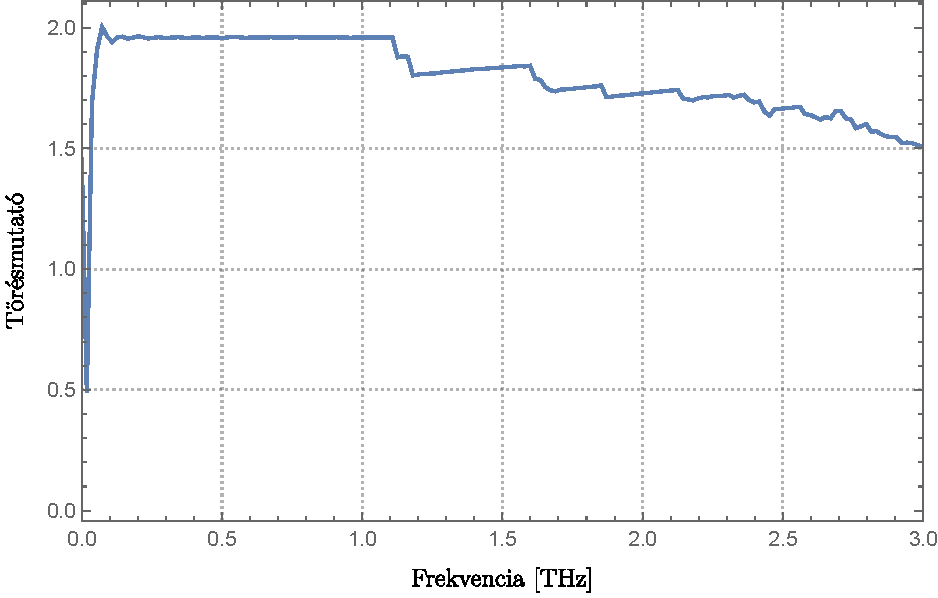
\includegraphics[width=0.7\linewidth]{beszamolo/tor1.pdf}




\end{center}
\caption{Számított törésmutató spektrum}

\label{fig:tor}
\end{figure}

Itt azt tapasztaltam hogy az irodalmi $n = 1.95_{f = 1\,THz}$ \cite{naftaly2021terahertz} értékkel hibahatáron belül megegyezik a mérésem.



\begin{figure}[H]
\begin{center}


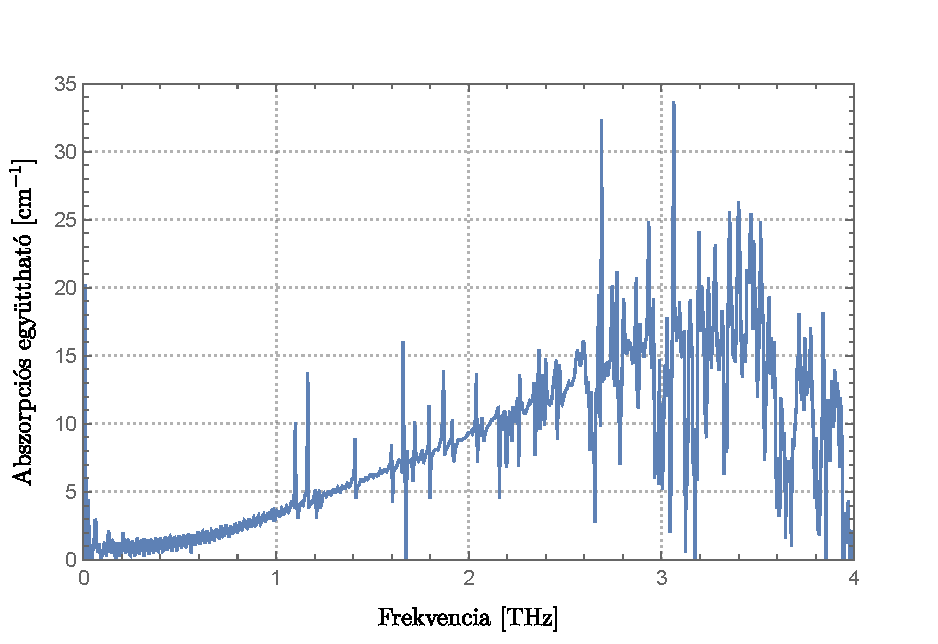
\includegraphics[width=0.7\linewidth]{beszamolo/absz1.pdf}




\end{center}
\caption{Számított abszorpció spektrum}

\label{fig:absz}
\end{figure}

\noindent A transzmisszó, abszorpciós együttható, és törésmutató spektrumokból azt a tanulságot lehet levonni hogy az ablak megfelelő intenzitást enged át 0-2 THz között ahol a vizsgálandó rezonancia van, így megfelelő jel-zaj viszony mellett lehet a kriosztáttal transzmissziós kísérleteket végezni.\\
A kutatásaimat a mintatartó pálca befejezésével és nagy mágneses terekben a minta spingerjesztéseinek vizsgálatával fogom folytatni.





\newpage

\printbibliography

\end{document}










